\documentclass{article}
	\usepackage{ctex}
    \usepackage{geometry}
        \geometry{left=2.54cm,right=2.54cm,top=2.54cm,bottom=2.54cm}
    \usepackage{longtable}
    \usepackage{booktabs}
    \usepackage{graphicx}
    \usepackage{extarrows}
    \begin{document}
	\title{数字逻辑与处理器基础大作业 \\ [2ex] \begin{large} \emph{单周期处理器} \end{large} }
	\author{王晗\\(2013011076)}
	\date{\today}
	\maketitle
	\section{处理器结构}
		\subsection{回答问题}
            \subsubsection*{1.由RegDst信号控制的多路选择器,输入2对应常数31。这里的31代表什么?在执行哪些指令时需要RegDst 信号为2?为什么?}
            31代表31号寄存器(\$ra)。

            在执行jal指令时需要RegDst信号为2,将当前指令的下一句的指令存储器地址写入\$ra寄存器,供程序跳转返回时使用。\\
            (教材附录中说,jalr中的rd默认值为31,当未指定rd时,由汇编器将rd置为31,或者由硬件将RegDst设为2。)
            \subsubsection*{2.由ALUSrc1信号控制的多路选择器,输入1对应的指令[10-6]是什么?在执行哪些指令时需要ALUSrc1信号为1?为什么?}
            指令[10-6]是移位偏移量shamt[4:0]。

            在执行sll、srl、sra指令时需要将ALUSrc1信号置为1,因为这些指令涉及移位操作,需要通过shamt[4:0]传入移位量。
            \subsubsection*{3.由MemtoReg信号控制的多路选择器,输入2对应的是什么?在执行哪些指令时需要MemtoReg信号为2?为什么?}
            MemtoReg为2时,表示将当前指令的下一句的指令存储器地址送入寄存器对写入数据总线。

            在执行jal、jalr指令时需要MemtoReg信号为2,将当前指令的下一句的指令存储器地址写入\$ra寄存器,供程序跳转返回时使用。
            \subsubsection*{4.图中的处理器结构并没有Jump控制信号,取而代之的是PCSrc信号。PCSrc信号控制的多路选择器,输入2对应的是什么?在执行哪些指令时需要PCSrc信号为2?为什么?}
            PCSrc信号为2时,表示将寄存器堆输出数据总线1上的数据作为下一条指令的指令存储器地址。

            在执行jr、jalr指令时,需要PCSrc信号为2,根据寄存器存储的地址进行跳转。
            \subsubsection*{5.为什么需要ExtOp控制信号?什么情况下ExtOp信号为1?什么情况下ExtOp信号为0?}
            将16位数扩展为32位时,存在无符号扩展和有符号扩展两种扩展方式。

            用最高位(符号位)填充高位时,ExtOp为1;否则ExtOp为0。
            \subsubsection*{6.若想再多实现一条指令nop(空指令),指令格式为全0,需要如何修改处理器结构?}
            空指令可以用sll \$0,\$0,0实现。不必改动现有的数据通路,只需将nop解释为从0号寄存器取值,左移0位,再存入0号寄存器即可。
        \subsection{填写真值表}
            \begin{longtable}{cccccccccccc}
                \multicolumn{12}{r}{接上页} \\
                \toprule
                 \rotatebox{65}{Instruction} & \rotatebox{65}{PCSrc[1:0]} & \rotatebox{65}{Branch} & \rotatebox{65}{RegWrite} & \rotatebox{65}{RegDst[1:0]} & \rotatebox{65}{MemRead} & \rotatebox{65}{MemWrite} & \rotatebox{65}{MemtoReg[1:0]} & \rotatebox{65}{ALUSrc1} & \rotatebox{65}{ALUSrc2} & \rotatebox{65}{ExtOp} & \rotatebox{65}{LuOp} \\
                \midrule
                \endhead
                \toprule
                 \rotatebox{65}{Instruction} & \rotatebox{65}{PCSrc[1:0]} & \rotatebox{65}{Branch} & \rotatebox{65}{RegWrite} & \rotatebox{65}{RegDst[1:0]}
                 & \rotatebox{65}{MemRead} & \rotatebox{65}{MemWrite} & \rotatebox{65}{MemtoReg[1:0]} & \rotatebox{65}{ALUSrc1}
                 & \rotatebox{65}{ALUSrc2} & \rotatebox{65}{ExtOp} & \rotatebox{65}{LuOp} \\
                \midrule
                \endfirsthead
                \bottomrule
                \multicolumn{12}{r}{转下页\dots} \\
                \endfoot
                \bottomrule
                \endlastfoot
                lw    & 0 & 0 & 1 & 0 & 1 & 0 & 1 & 0 & 1 & 1 & 0 \\
                sw    & 0 & 0 & 0 & x & 0 & 1 & x & 0 & 1 & 1 & 0 \\
                lui   & 0 & 0 & 1 & 0 & 0 & 0 & 0 & 0 & 1 & x & 1 \\
                add   & 0 & 0 & 1 & 1 & 0 & 0 & 0 & 0 & 0 & x & x \\
                addu  & 0 & 0 & 1 & 1 & 0 & 0 & 0 & 0 & 0 & x & x \\
                sub   & 0 & 0 & 1 & 1 & 0 & 0 & 0 & 0 & 0 & x & x \\
                subu  & 0 & 0 & 1 & 1 & 0 & 0 & 0 & 0 & 0 & x & x \\
                addi  & 0 & 0 & 1 & 0 & 0 & 0 & 0 & 0 & 1 & 1 & 0 \\
                addiu & 0 & 0 & 1 & 0 & 0 & 0 & 0 & 0 & 1 & 0 & 0 \\
                and   & 0 & 0 & 1 & 1 & 0 & 0 & 0 & 0 & 0 & x & x \\
                or    & 0 & 0 & 1 & 1 & 0 & 0 & 0 & 0 & 0 & x & x \\
                xor   & 0 & 0 & 1 & 1 & 0 & 0 & 0 & 0 & 0 & x & x \\
                nor   & 0 & 0 & 1 & 1 & 0 & 0 & 0 & 0 & 0 & x & x \\
                andi  & 0 & 0 & 1 & 0 & 0 & 0 & 0 & 0 & 1 & 0 & 0 \\
                sll   & 0 & 0 & 1 & 1 & 0 & 0 & 0 & 1 & 0 & x & x \\
                srl   & 0 & 0 & 1 & 1 & 0 & 0 & 0 & 1 & 0 & x & x \\
                sra   & 0 & 0 & 1 & 1 & 0 & 0 & 0 & 1 & 0 & x & x \\
                slt   & 0 & 0 & 1 & 1 & 0 & 0 & 0 & 0 & 0 & x & x \\
                sltu  & 0 & 0 & 1 & 1 & 0 & 0 & 0 & 0 & 0 & x & x \\
                slti  & 0 & 0 & 1 & 0 & 0 & 0 & 0 & 0 & 1 & 1 & 0 \\
                sltiu & 0 & 0 & 1 & 0 & 0 & 0 & 0 & 0 & 1 & 0 & 0 \\
                beq   & 0 & 1 & 0 & x & 0 & 0 & x & 0 & 0 & 1 & 0 \\
                j     & 1 & x & 0 & x & 0 & 0 & x & x & x & x & x \\
                jal   & 1 & x & 1 & 2 & 0 & 0 & 2 & x & x & x & x \\
                jr    & 2 & x & 0 & x & 0 & 0 & x & x & x & x & x \\
                jalr  & 2 & x & 1 & 1 & 0 & 0 & 2 & x & x & x & x
            \end{longtable}
    \section{完成控制器}
        \subsection{阅读CPU.v}
        \subsection{完成Control.v}
            \emph{见文件Control.v。}
        \subsection{阅读InstructionMemory.v}
            \subsubsection*{这段程序执行足够长时间后会发生什么?}
            程序停在Loop: j Loop语句。
            \subsubsection*{此时寄存器\$a0\~{}\$a3,\$t0\~{}\$t2,\$v0\~{}\$v1中的值应是多少?写出计算过程。}
            \texttt{\begin{tabular}{rll}
                & addi \$a0, \$zero, 12345 & \$a0=0x00003039 \\
                & addiu \$a1, \$zero, -11215 & \$a1=0x0000d431 \\
                & sll \$a2, \$a1, 16 & \$a2=0xd4310000 \\
                & sra \$a3, \$a2, 16 & \$a3=0xffffd431 \\
                & beq \$a3, \$a1, L1 & \$a3$\not=$\$a1 \\
                & lui \$a0, -11111 &  \$a0=0xd4990000 \\
                L1: & add \$t0, \$a2, \$a0 & \$t0=0xa8ca0000 \\
                & sra \$t1, \$t0, 8 & \$t1=0xffa8ca00 \\
                & addi \$t2, \$zero, -12345 & \$t2=0xffffcfc7 \\
                & slt \$v0, \$a0, \$t2 & \$a0<\$t2<0, 故\$v0=0x00000001 \\
                & sltu \$v1, \$a0, \$t2 & 0<\$a0<\$t2, 故\$v1=0x00000001\\
                Loop: & j Loop &  \\
            \end{tabular}}
            \subsubsection*{如果已知某一时刻在某寄存器中存放着数0xffffcfc7,能否判断出它是有符号数还是无符号数?为什么?}
            不能。0xffffcfc7可能表示无符号数4294954951,也有可能表示有符号数-12345。无符号数和有符号数在寄存器中不可区分,最高位是否当作符号位由指令决定。
        \subsection{ModelSim仿真}
            \subsubsection*{PC如何变化?}
            每个时钟周期PC的值增加4,当PC达到0x2c(仿真时间1100ns)后保持不变。
            \subsubsection*{Branch信号在何时为1?它引起了PC怎样的变化?}
            PC=0x10(仿真时间400ns)时Branch信号为1。但由于Zero信号仍为0,PC移向下一条指令(PC<=PC+4)。
            \subsubsection*{100\~{}200ns期间,PC是多少?对应的指令是哪条?此时\$a1的值是多少?200\~{}300ns期间\$a1的值是多少?为什么会这样?下一条指令立即使用到了\$a1的值,会出现错误吗?为什么?}
            100\~{}200ns期间PC=0x04,对应指令addiu \$a1, \$zero, -11215,此时\$a1=0x00000000,200\~{}300ns期间\$a1=0x0000d431。

            寄存器写入只发生在时钟沿上。100ns上升沿时,写入信号还未产生,因此需要等到下一个上升沿才能写入寄存器\$a1。

            下一条指令立即使用\$a1的值并不会出现错误,\$a1将在时钟上升沿到来时立刻写入,寄存器写入的延时远小于下一条指令从指令存储器读出、译码产生控制信号、选择数据通路等消耗的时间。
            \subsubsection*{运行时间足够长之后(如1100ns时)寄存器\$a0\~{}\$a3,\$t0\~{}\$t2,\$v0\~{}\$v1中的值是多少?与你的预期是否一致?}
            \begin{figure}[htb]
                \centering
                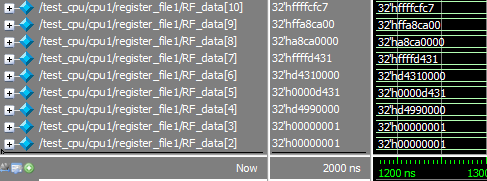
\includegraphics{fig1.png} \\
                \caption{\label{fig:reg-value-1}ASM1运行足够长时间后寄存器中的值}
            \end{figure}
            从上图可以看出,ModelSim仿真结果与计算结果一致。
    \section{执行汇编程序}
        \subsection{阅读并理解汇编程序}
            \subsubsection*{如果第一行的3是任意正整数n,这段程序能实现什么功能?}
            求$\sum_{i=1}^{n}{i}$.
            \subsubsection*{Loop、sum、L1各有什么作用?}
            Loop、sum、L1是Label,用来标记指令地址,供汇编器在翻译跳转、分支指令机器码时使用。

            本例中,Loop是程序运行结束后停止的位置;sum是递归深度增加时压栈操作开始的位置;L1是递归深度控制变量\$a0改变的位置,其后的语句完成了继续递归、回溯弹栈、计算返回值等功能。
            \subsubsection*{为每一句代码添加注释。}
            \texttt{\begin{tabular}{rll}
                & addi \$a0, \$zero, 3 & \$a0=3 \\
                & jal sum & 跳转至sum,并修改\$ra \\
                Loop: & beq \$zero, \$zero, Loop & 停止在Loop处 \\
                sum: & addi \$sp, \$sp, -8 & 栈指针下移2个字 \\
                & sw \$ra, 4(\$sp) & \$ra入栈 \\
                & sw \$a0, 0(\$sp) &  \$a0入栈 \\
                & slti \$t0, \$a0, 1 & \$t0 = \$a0 < 1 \\
                & beq \$t0, \$zero, L1 & \~{}\$t0则跳转至L1继续递归 \\
                & xor \$v0, \$zero, \$zero & \$v0清零 \\
                & addi \$sp, \$sp, 8 & 栈指针上移2个字 \\
                & jr \$ra & 根据\$ra存储的地址返回 \\
                L1: & addi \$a0, \$a0, -1 & \$a0-- \\
                & jal sum & 跳转至sum,并修改\$ra \\
                & lw \$a0, 0(\$sp) & \$a0出栈 \\
                & lw \$ra, 4(\$sp) & \$ra出栈 \\
                & addi \$sp, \$sp, 8 & 栈指针上移2个字 \\
                & add \$v0, \$a0, \$v0 & \$v0 = \$a0 + \$v0\\
                & jr \$ra & 根据\$ra存储的地址返回 \\
            \end{tabular}}

        \subsection{将汇编程序翻译为机器码}
            \subsubsection*{对于beq和jal语句中的Loop,sum,L1,你是怎么翻译的?立即数-1、-8被翻译成了什么(用16进制或2进制表示)?}
            beq语句中的地址字段是目标位置相对当前指令的下一条指令位置的偏移量(字数),因此beq \$zero, \$zero, Loop中的Loop应当翻译为-1,beq \$t0, \$zero, L1中的L1应当翻译为3。

            jal语句中的地址字段是目标地址的[27:2]位,因此jal sum中的sum应当翻译为0x0000003。

            立即数-1翻译为0xffff,-8翻译为0xfff8。

            翻译后的机器码对应如下:

            \texttt{\begin{tabular}{rll}
                & addi \$a0, \$zero, 3 & \{6'h08, 5'd00, 5'd04, 16'h0003\}; \\
                & jal sum & \{6'h03, 26'h0000003\}; \\
                Loop: & beq \$zero, \$zero, Loop & \{6'h04, 5'd00, 5'd00, 16'hffff\}; \\
                sum: & addi \$sp, \$sp, -8 & \{6'h08, 5'd29, 5'd29, 16'hfff8\}; \\
                & sw \$ra, 4(\$sp) & \{6'h2b, 5'd29, 5'd31, 16'h0004\}; \\
                & sw \$a0, 0(\$sp) & \{6'h2b, 5'd29, 5'd04, 16'h0000\}; \\
                & slti \$t0, \$a0, 1 & \{6'h0a, 5'd04, 5'd08, 16'h0001\}; \\
                & beq \$t0, \$zero, L1 & \{6'h04, 5'd00, 5'd08, 16'h0003\}; \\
                & xor \$v0, \$zero, \$zero & \{6'h00, 5'd00, 5'd00, 5'd02, 5'd00, 6'h26\}; \\
                & addi \$sp, \$sp, 8 & \{6'h08, 5'd29, 5'd29, 16'h0008\}; \\
                & jr \$ra & \{6'h00, 5'd31, 15'h0000, 6'h08\}; \\
                L1: & addi \$a0, \$a0, -1 & \{6'h08, 5'd04, 5'd04, 16'hffff\}; \\
                & jal sum & \{6'h03, 26'h0000003\}; \\
                & lw \$a0, 0(\$sp) & \{6'h23, 5'd29, 5'd04, 16'h0000\}; \\
                & lw \$ra, 4(\$sp) & \{6'h23, 5'd29, 5'd31, 16'h0004\}; \\
                & addi \$sp, \$sp, 8 & \{6'h08, 5'd29, 5'd29, 16'h0008\}; \\
                & add \$v0, \$a0, \$v0 & \{6'h00, 5'd04, 5'd02, 5'd02, 5'd00, 6'h20\}; \\
                & jr \$ra & \{6'h00, 5'd31, 15'h0000, 6'h08\}; \\
            \end{tabular}}
        \subsection{ModelSim仿真}
            \subsubsection*{运行时间足够长之后(如5000ns时),寄存器\$a0,\$v0的值是多少?和你预期的程序功能是否一致?}
            \begin{figure}[htb]
                \centering
                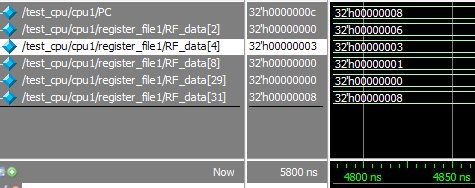
\includegraphics{fig2.png} \\
                \caption{\label{fig:reg-value-2}ASM2运行足够长时间后寄存器中的值}
            \end{figure}
            从图中可以看出,运行足够长时间后,\$a0=3, \$v0=6, 和预期功能一致。
            \subsubsection*{观察、描述并解释PC,\$a0,\$v0,\$sp,\$ra如何变化。}
            PC的变化:除跳转外,每个时钟周期PC<=PC+4。 \\
            \texttt{
            0x00 $\rightarrow$ 0x04 $\xrightarrow{\text{跳转至sum}}$ 0x0c $\rightarrow$ 0x10  $\rightarrow$ 0x14 $\rightarrow$ 0x18 $\rightarrow$ 0x1c $\xrightarrow{\text{跳转至L1}}$ 0x2c $\rightarrow$ 0x30 $\xrightarrow{\text{跳转至sum}}$ 0x0c $\rightarrow$ 0x10 $\rightarrow$ 0x14 $\rightarrow$ 0x18 $\rightarrow$ 0x1c $\xrightarrow{\text{跳转至L1}}$ 0x2c $\rightarrow$ 0x30 $\xrightarrow{\text{跳转至sum}}$ 0x0c $\rightarrow$ 0x10  $\rightarrow$ 0x14 $\rightarrow$ 0x18 $\rightarrow$ 0x1c $\xrightarrow{\text{跳转至L1}}$ 0x2c $\rightarrow$ 0x30 $\xrightarrow{\text{跳转至sum}}$ 0x0c $\rightarrow$ 0x10 $\rightarrow$ 0x14 $\rightarrow$ 0x18 $\rightarrow$ 0x1c $\rightarrow$ 0x20 $\rightarrow$ 0x24 $\rightarrow$ 0x28 $\xrightarrow{\text{跳转至\$ra}}$ 0x34 $\rightarrow$ 0x38 $\rightarrow$ 0x3c $\rightarrow$ 0x40 $\rightarrow$ 0x44 $\xrightarrow{\text{跳转至\$ra}}$ 0x34 $\rightarrow$ 0x38 $\rightarrow$ 0x3c $\rightarrow$ 0x40 $\rightarrow$ 0x44 $\xrightarrow{\text{跳转至\$ra}}$ 0x34 $\rightarrow$ 0x38 $\rightarrow$ 0x3c $\rightarrow$ 0x40 $\rightarrow$ 0x44 $\xrightarrow{\text{跳转至\$ra}}$ 0x08
            ~\\}

            \$a0的变化: \\
            \texttt{
            0x00 $\xrightarrow{\text{+3}}$ 0x03 $\xrightarrow{\text{压栈, -1}}$ 0x02 $\xrightarrow{\text{压栈, -1}}$ 0x01 $\xrightarrow{\text{压栈, -1}}$ 0x00 $\xrightarrow{\text{弹栈}}$ 0x01 $\xrightarrow{\text{弹栈}}$ 0x02 $\xrightarrow{\text{弹栈}}$ 0x03
            ~\\}

            \$v0的变化: \\
            \texttt{
            0x00 $\xrightarrow{\text{清零}}$ 0x00 $\xrightarrow[\text{第3层递归, 回溯}]{\text{+\$a0}}$ 0x01 $\xrightarrow[\text{第2层递归, 回溯}]{\text{+\$a0}}$ 0x03 $\xrightarrow[\text{第1层递归, 回溯}]{\text{+\$a0}}$ 0x06
            ~\\}

            \$sp的变化: \\
            \texttt{
            0x00 $\xrightarrow[\text{第1层递归}]{\text{-8}}$ 0xf8 $\xrightarrow[\text{第2层递归}]{\text{-8}}$ 0xf0 $\xrightarrow[\text{第3层递归}]{\text{-8}}$ 0xe8 $\xrightarrow[\text{第4层递归}]{\text{-8}}$ 0xe0 \\
            $\xrightarrow[\text{第4层递归, 回溯}]{\text{+8}}$ 0xe8 $\xrightarrow[\text{第3层递归, 回溯}]{\text{+8}}$ 0xf0 $\xrightarrow[\text{第2层递归, 回溯}]{\text{+8}}$ 0xf8 $\xrightarrow[\text{第1层递归, 回溯}]{\text{+8}}$ 0x00
            ~\\}

            \$ra的变化: \\
            \texttt{
            0x00 $\xrightarrow[\text{\$ra<=Line2Addr}]{\text{Line1: jal sum}}$ 0x08 $\xrightarrow[\text{第1层递归}]{\text{压栈}}$ $\xrightarrow[\text{\$ra<=Line13Addr}]{\text{Line12: jal sum}}$ 0x34 $\xrightarrow[\text{第2层递归}]{\text{压栈}}$ $\xrightarrow[\text{\$ra<=Line13Addr}]{\text{Line12: jal sum}}$ 0x34 $\xrightarrow[\text{第3层递归}]{\text{压栈}}$ $\xrightarrow[\text{\$ra<=Line13Addr}]{\text{Line12: jal sum}}$ 0x34 $\xrightarrow[\text{第4层递归}]{\text{压栈}}$ $\xrightarrow{\text{丢弃栈顶}}$ $\xrightarrow{\text{弹栈}}$ 0x34 $\xrightarrow{\text{弹栈}}$ 0x34 $\xrightarrow{\text{弹栈}}$ 0x08
            }

\end{document} 